\subsection{MedQA}
{{\footnotesize
\noindent MedQA is a large-scale multiple-choice dataset drawn from professional medical
board exams (e.g., USMLE), testing AI systems on diagnostic and medical knowledge 
questions in English and Chinese.


\begin{description}[labelwidth=4cm, labelsep=1em, leftmargin=4cm, itemsep=0.1em, parsep=0em]
  \item[date:] 2020-09-28
  \item[version:] 1
  \item[last\_updated:] 2020-09-28
  \item[expired:] false
  \item[valid:] yes
  \item[valid\_date:] 2020-09-28
  \item[url:] \href{https://arxiv.org/abs/2009.13081}{https://arxiv.org/abs/2009.13081}
  \item[doi:] 10.48550/arXiv.2009.13081
  \item[domain:] Medical Question Answering
  \item[focus:] Medical board exam QA
  \item[keywords:]
    - USMLE
    - diagnostic QA
    - medical knowledge
    - multilingual
  \item[licensing:] Under Association for the Advancement of Artificial Intelligence
  \item[task\_types:]
    - Multiple choice
  \item[ai\_capability\_measured:]
    - Medical diagnosis and knowledge retrieval
  \item[metrics:]
    - Accuracy
  \item[models:]
    - Neural reader
    - Retrieval-based QA systems
  \item[ml\_motif:]
    - Medical diagnosis
  \item[type:] Benchmark
  \item[ml\_task:]
    - Supervised Learning
  \item[solutions:] 0
  \item[notes:] Multilingual (English, Simplified and Traditional Chinese)
  \item[contact.name:] Di Jin
  \item[contact.email:] jindi15@mit.edu
  \item[datasets.links.name:] Github
  \item[datasets.links.url:] \href{https://github.com/jind11/MedQA}{https://github.com/jind11/MedQA}
  \item[results.links.name:] unknown
  \item[results.links.url:] \href{unknown}{unknown}
  \item[fair.reproducible:] True
  \item[fair.benchmark\_ready:] True
  \item[id:] medqa
  \item[Citations:] \cite{jin2020diseasedoespatienthave}
\end{description}

{\bf Ratings:} ~ \\

\begin{tabular}{p{0.15\textwidth} p{0.07\textwidth} p{0.7\textwidth}}
\hline
Rating & Value & Reason \\
\hline
dataset & 4 & Dataset is publicly available (GitHub, paper, Hugging Face), well-structured. However, versioning and metadata could be more standardized to fully meet FAIR criteria.
 \\
documentation & 4 & Paper is available. Evaluation criteria are not mentioned.
 \\
metrics & 5 & Uses clear, quantitative metric (accuracy), standard for multiple-choice benchmarks; easily comparable across models.
 \\
reference\_solution & 0 & No reference solution mentioned.
 \\
software & 5 & All code available on the github
 \\
specification & 3 & Task is clearly defined as multiple-choice QA for medical board exams; input and output formats are explicit; task scope is rigorous and structured. System constraints not specified.
 \\
\hline
\end{tabular}

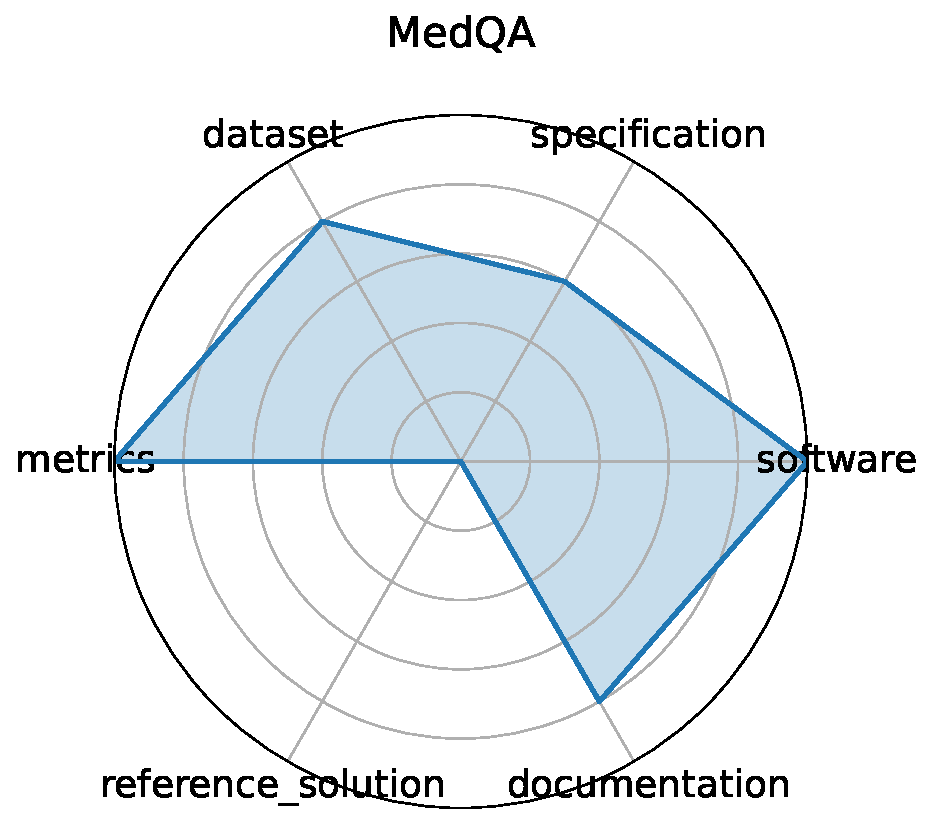
\includegraphics[width=0.2\textwidth]{medqa_radar.pdf}
}}
\clearpage